\documentclass[11pt]{article}
\usepackage{geometry}                % See geometry.pdf to learn the layout options. There are lots.
\geometry{letterpaper}                   % ... or a4paper or a5paper or ... 
%\geometry{landscape}                % Activate for for rotated page geometry
%\usepackage[parfill]{parskip}    % Activate to begin paragraphs with an empty line rather than an indent
\usepackage{graphicx}
\usepackage{color}
\usepackage{amssymb}
\usepackage{epstopdf}
\usepackage{sectsty}
\usepackage[hyphens]{url}  %% be sure to specify the option 'hyphens'
\DeclareGraphicsRule{.tif}{png}{.png}{`convert #1 `dirname #1`/`basename #1 .tif`.png}

\title{Drake-Cullen-Part-A-Answers}
\author{Drake Cullen}
%\date{}                                           % Activate to display a given date or no date

\begin{document}
%\maketitle
%\section{}
%\subsection{}
\begin{minipage}{\linewidth}% to keep image and caption on one page
\centering

\includegraphics[keepaspectratio=true,scale=0.35]{CMU.png}
\end{minipage}
\section*{ \centering Part A Answers}
\subsection*{ \centering By Drake Cullen} 

\vspace{5mm}
 
I declare that all material in this assessment task is my work except where there is clear acknowledgement or reference to the work of others. I further declare that I have complied and agreed to the CMU Academic Integrity Policy at the University website. http://www.coloradomesa.edu/student-services/documents
\begin{center}
\textbf{Author’s Name:} Drake Cullen 
\textbf{UID(700\#):} 700480375
\textbf{ Date:} 10/17/2021
\end{center} 

\section*{Statement a)}
I tested my hashtable with occupancy ratios of 50\%, 70\%, and 80\%. For each occupancy ratio, 7,650,000 lookups were performed with random words so that a discernable time difference could be found. \newline The occupancy ratio of 50\% took 1,072,580 clock cycles and 1.07223 seconds to perform the lookups. There were 1,650 collisions. \newline The occupancy ratio of 70\% took 1,091,944 clock cycles and 1.09161 seconds to perform the lookups. There were 1,898 collisions. \newline The occupancy ratio of 80\% took 1,0122,989 clock cycles and 1.12265 seconds to perform the lookups. There were 2,049 collisions. \newline I decided to use an occupancy ratio of 50\% for the rest of my experiments.


\section*{Statement b)}
I used open hashing, so my hash table could handle variable sizes by adding new elements to the linked list.

\section*{Statement c)}
I started off with the hash function f(r) = r \% hsize. Next, I incorporated the following hash function from our slides:

\begin{center}
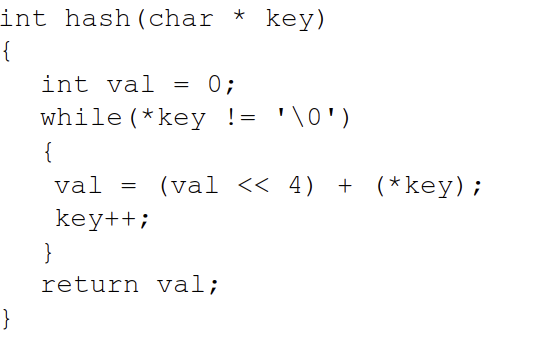
\includegraphics[keepaspectratio=true,scale=0.5]{slides-hash.png}
\end{center}

In order to minimize collisions, I created a set of nested loops to change the initial val to numbers in the range from 0 to 10,000. Every time I changed the initial value, the bit shifting variable looped through values of 0 to 25. In the end, I found an initial value of 530 with a left shift of 8 minimized the number of collisions.

\section*{Statement d)}
If there is a collision, I iterate over the corresponding linked list and insert the new word in alphabetical order.

\section*{Statement e)}
No, you don't need an interface class for each function. I put my hashtable in a class, so I did use an interface class for the hashtable methods.

\end{document}  